\subsubsection{LEGO MINDSTORMS EV3 (ID: 95646)}
\begin{figure}[H]
  \centering
  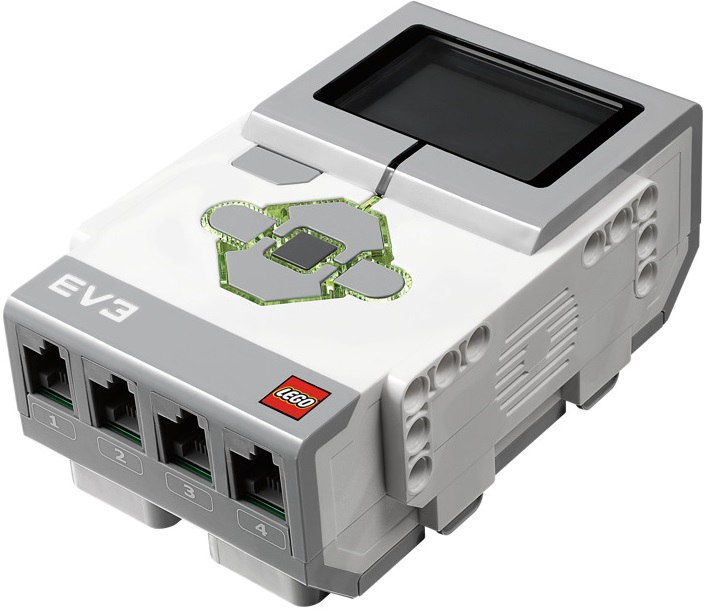
\includegraphics[width=4cm]{images/techAnalysis/LegoEV3.jpg}
  \caption{LEGO MINDSTORMS EV3 brick \cite{BrickOWl-figure-EV3}}\label{fig:sssec:LEGOEV3-EV3}
\end{figure}
The LEGO MINDSTORMS is about creating and programming robots to do different tasks.
The key component in this is the EV3 brick, which is a programmable computer, that can be connected to sensors and motors, in order to accomplish its tasks.
It's driven by a 300MHz 32bit ARM9 processor, 64MB of RAM and 16MB FLASH memory, which can be extended with the built-in SDHC-card reader.
The brick has four ports to read input from devices such as touch-sensor, gyro sensor or any of the others compatible sensors within the LEGO universe.
The brick also has four output ports for motors.
The cables for all the input and output ports are RJ12, which are the cables used for the different sensors and motors within the MINDSTORMS brand of LEGO, and there exist converter cables to other LEGO motors, such as the LEGO Technic motors \cite{LEGO_ev3_nodate}.
The connection to the EV3 can be done by either Bluetooth, USB-port, or WIFI, depending on what the user considers as the most optimal.
The brick also allows for controlling through the physical buttons on the brick itself, where the 178x128 pixel built-in display provides information.
The Ev3 brick also allow sound output through its built-in speakers.
Furthermore, it can be powered by a power supply, or by battery; either six AA batteries or the LEGO MINDSTORMS EV3 rechargeable DC Battery which is a 2050mAh lithium-ion battery \cite{LEGO_lego_nodate2}. \cite{LEGO_mindstorms_2013-1} \cite{LEGO_lego_nodate}
